\subsection{Water governance regimes}
\label{Res.1}

\begin{figure*}[ht!]
	\centering
	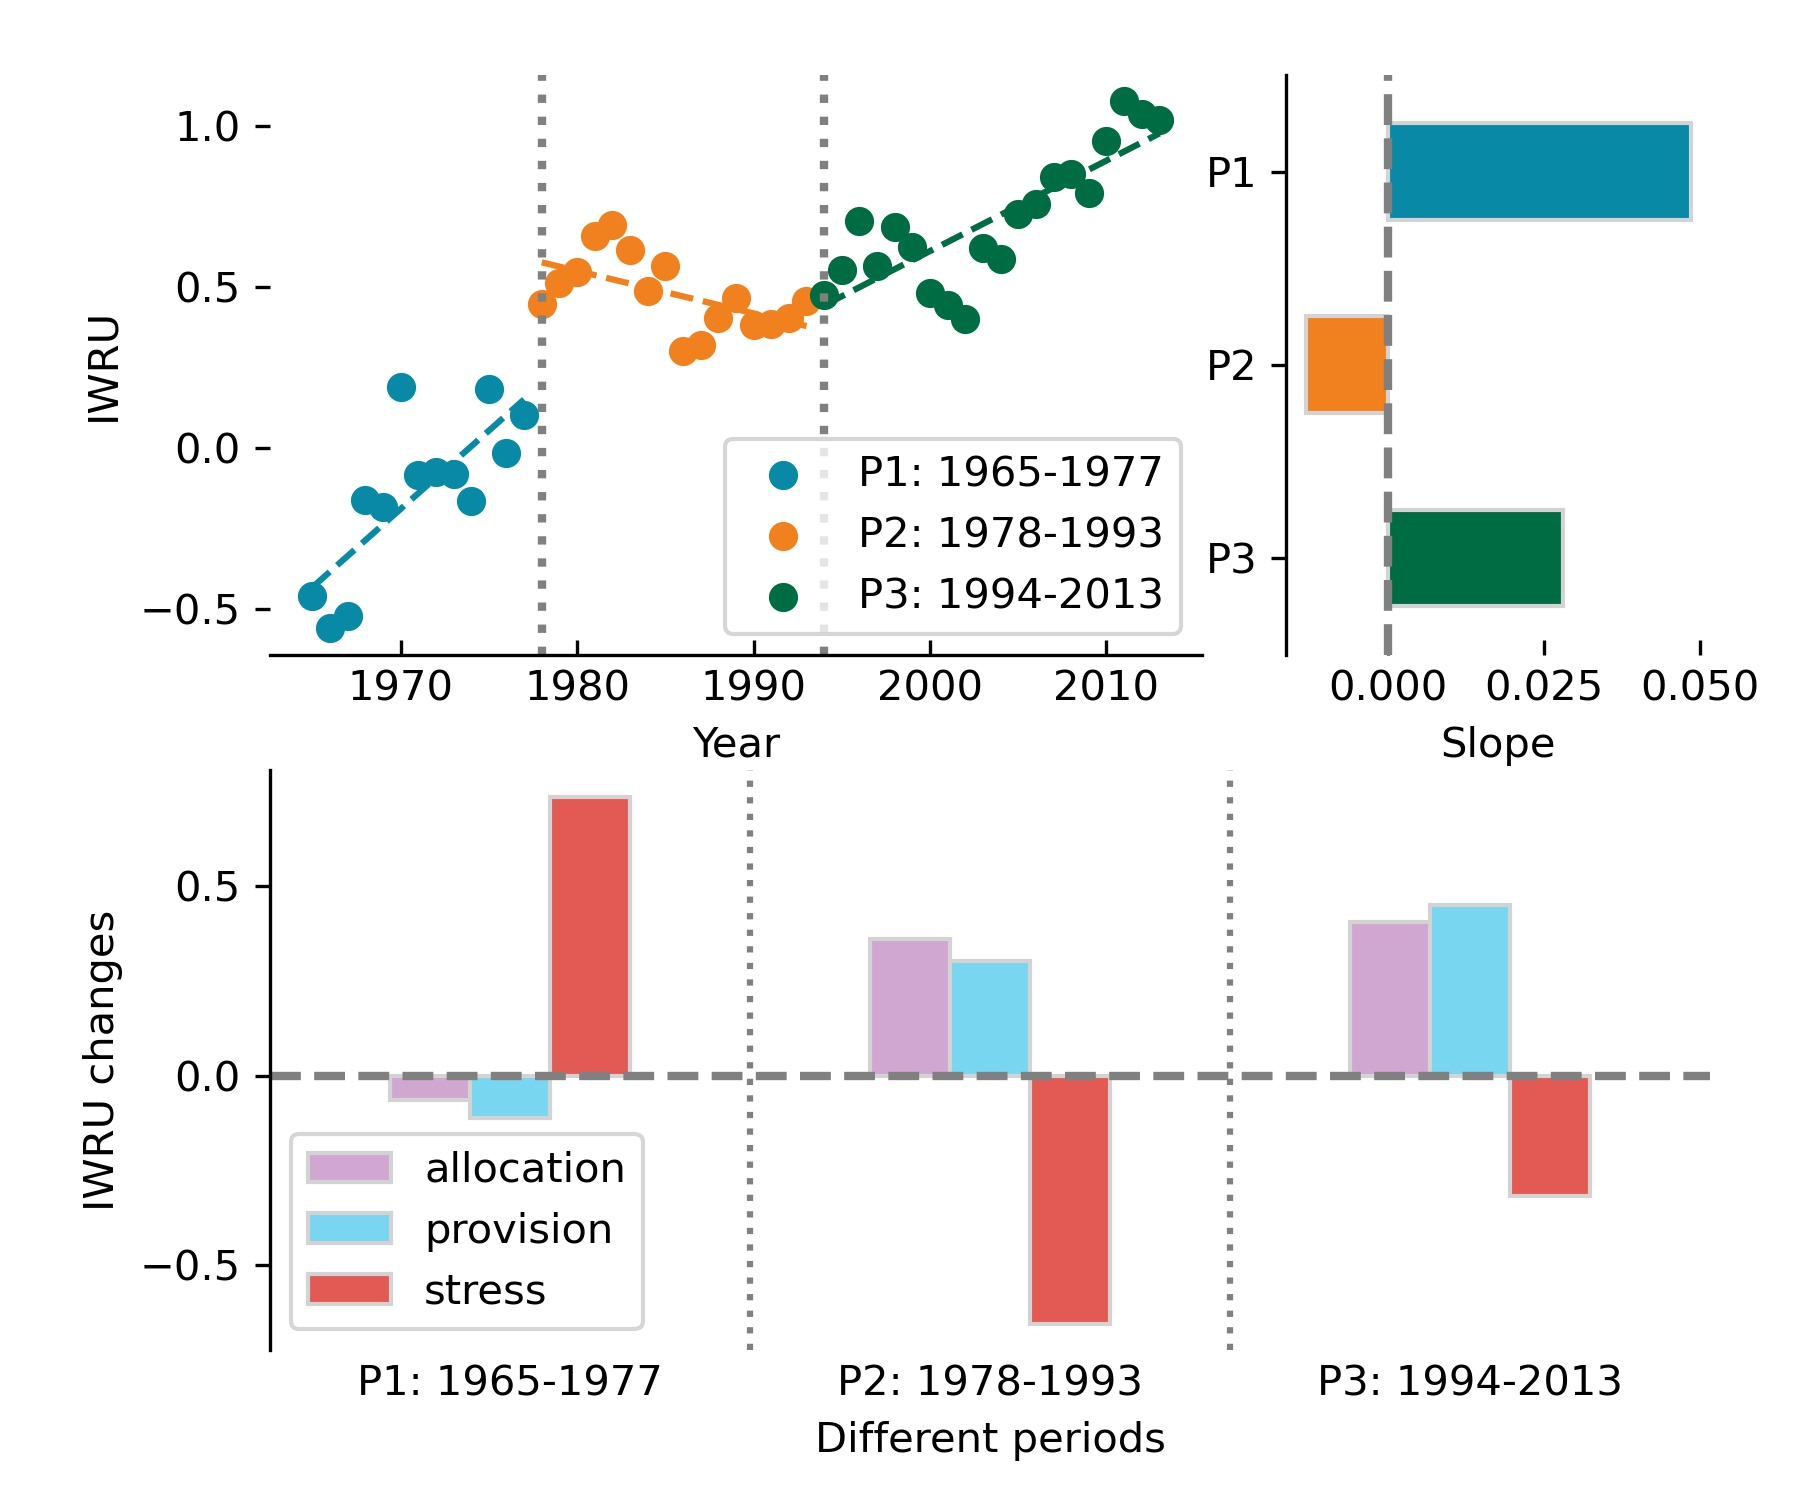
\includegraphics[width=0.9\linewidth]{main/index.jpg}
	\caption{Changes in the IWGI index.
	\textbf{A,} Change points detection. With significant change points in 1978 and 1994, the IWGI has three different periods.
	\textbf{B,} Contributions of each dimension to the changes of IWGI within each of the three periods. Supply, purpose and allocation were the main positive contributors to P1, P2 and P3.
	\textbf{C,} Combination of contributions across three dimensions in different periods (S: supply; P: purpose; A: allocation). The closer a point is to an angle of the outside triangle, the greater the proportion of the contribution of this dimension.
	The red indicator line in this plot denotes a 1:1 contributions between purpose (P) and allocation (A). When the points are below this line, the contribution ratio of allocation is lower than that of function, and \textit{vice versa}.
	}
	\label{fig:IWGI}
\end{figure*}

% 这一节主要展示IWGI的变化趋势和WUR的划分
Two significant breakpoints divide the changes in the IWGI into three periods, with different contributions from three dimensions (Figure~\ref{fig:IWGI}A).
% 第一阶段
In the first period (P1, 1965-1978), the IWGI decreased rapidly.
While the indicator of purpose and allocation contributed more to the IWGI, the remarkable downward trend correlates significantly to the decreasing allocation and stress indicators (Figure~\ref{fig:IWGI}B).
% 第二阶段
In the second period (P2, 1979-2001), the increasing stress indicator significantly contributed to the upward IWGI, while the allocation and purpose indicators played negative roles in changing the IWGI.
% 第三阶段
During the third period (P3, 1995-2013), while the stress indicator kept its most significant share in contributions, the increased allocation indicator and decreased purpose indicator changed the regime of IWGI.

% 每个时期都有一个独特的、最引人注目的、对IWGI作出积极贡献的人。不同时期的三维总体特征如图所示。
Overall features of the three dimensions in different periods are shown in Ternary, where each regime shift associates to a directional change in the combination of three dimensions (Figure~\ref{fig:IWGI}C).
% 第一阶段到第二阶段
Throughout P1, the IWGI shifts paralleled with the left axis because the Purpose indicator was barely changed and others two changed in similar trends.
Analogously, as the stress indicator unchanged during the P3, the IWGI shifts paralleled with the right axis while others two changed in opposite trends.
% 第三阶段集中
The regime then experienced a long distance shift during the P2, as three indicators changed their ratios of contribution drastically to IWGI, simultaneously.
% 总结来说,三个稳态
The three different periods corresponded to three distinct water governance regimes: a massive supply regime (P1: 1965-1978), governance transforming regime (P2: 1979-2001), and a demand regulating regime (P3: 2002-2013).


% \begin{figure}[!htbp]
% 	\centering
% 	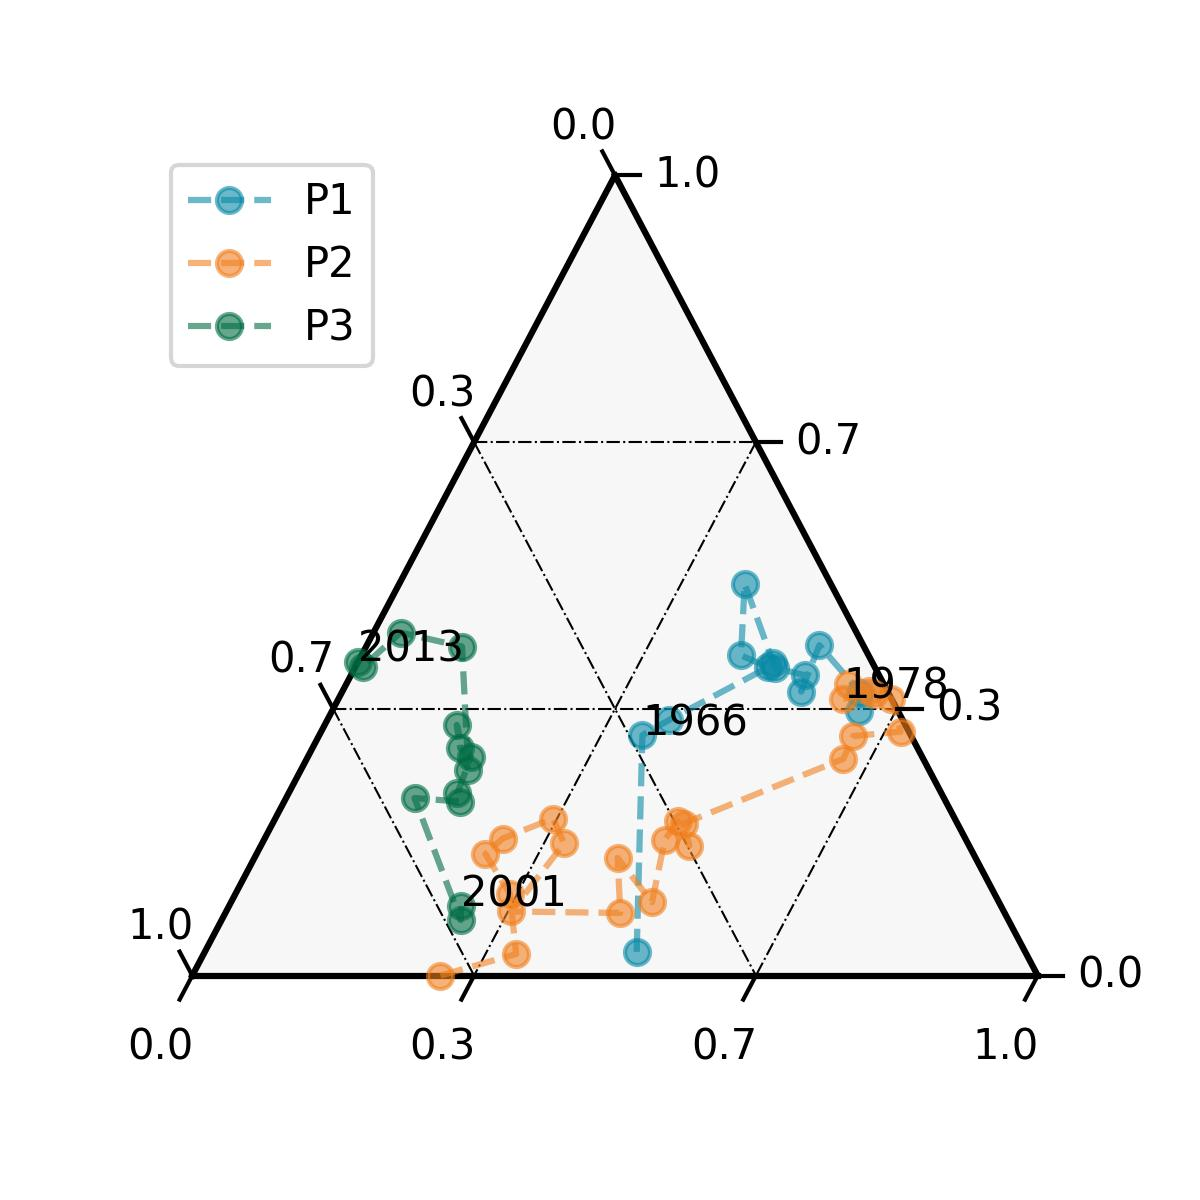
\includegraphics[width=0.9\linewidth]{main/phases.jpg}
% 	\caption{Combination of contributions across three dimensions in different periods (S: supply; P: purpose; A: allocation). The closer a point is to an angle of the outside triangle, the greater the proportion of the contribution of this dimension.
% 	The red indicator line in this plot denotes a 1:1 contributions between purpose (P) and allocation (A). When the points are below this line, the contribution ratio of allocation is lower than that of function, and \textit{vice versa}.}
% 	% 由于阶段一的点位于该线上方,L的净贡献比例多于P,而第二阶段的点则恰好相反。
% 	\label{fig:phases}
% \end{figure}

\subsection{Causes of water governance regime shifts}
\label{Res.2}

\begin{figure*}[th!]
	\centering
	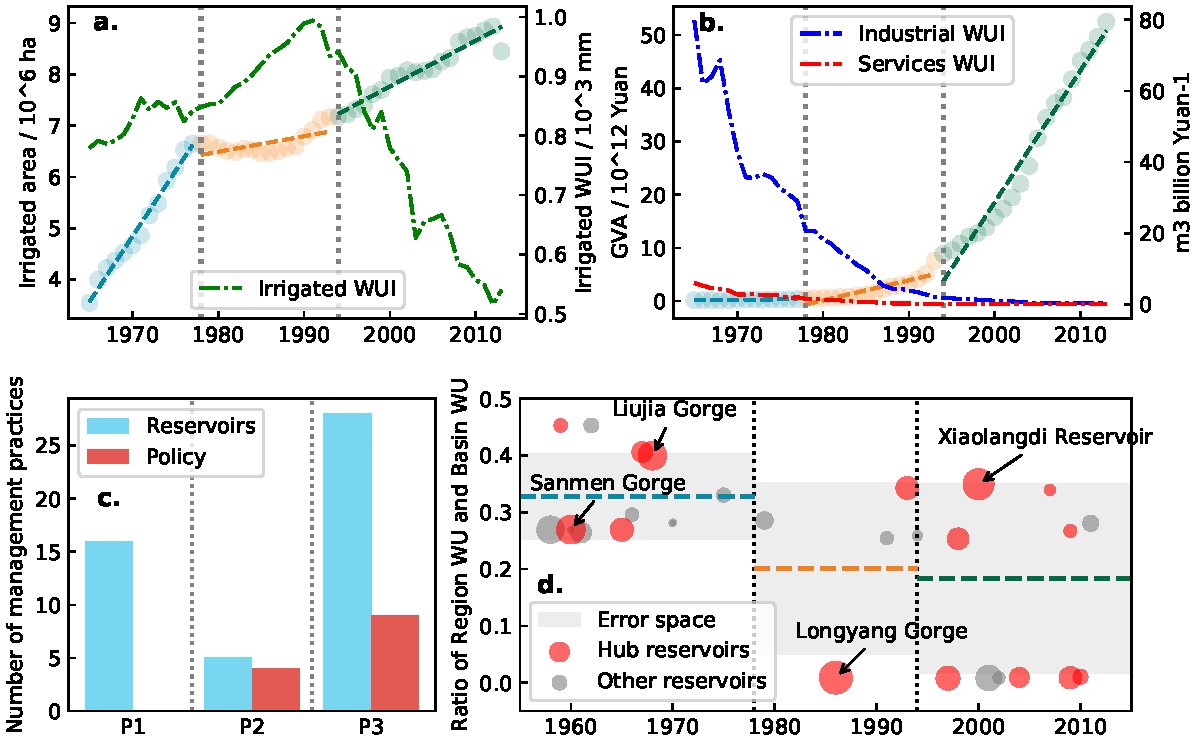
\includegraphics[width=0.9\linewidth]{main/causes.pdf}
	\caption{
		Causes of water governance regime shifts in the Yellow River Basin: environmental change, economic growth and efficiency changes, social transformation, and water governance policies.
		\textbf{A.} Changes in total irrigated area (orange line), and in water use intensity ($WU/A$, water use divided by the area, the green dot line), see \textit{SI Appendix} Methods S2).
		\textbf{B.} Changes in gross values added (GVA) of industry and services (blue line), and their water use intensities ($WU/GVA$ WU divided by the GVA, the red dot line) (\textit{SI Appendix} Methods S2).
		\textbf{C.} Completed time of each new reservoir and their located region's (source, upper, middle, or lower reaches) water use percentages as a proportion of the basin's total water use (WU) at that time. Red circles denote the reservoirs mainly for managing and regulating the whole basin.
		The size of each circle indicates the magnitude of its water storage capacity. Some important reservoirs include: (1) Xiaolangdi reservoir and Sanmen Reservoir, which were constructed mainly for managing sediments; and (2) Impoundments at Liujia Gorge, Longyang Gorge, which were constructed mainly for managing flood water discharge and water supply. The named reservoirs are significant for the entire basin, not only for regional development.
		%! 不清楚D的这些圆圈代表啥
		\textbf{D.} Social transformations and national-level policies related to water governance (see \textit{SI Appendix} Methods S1 and Table S2). In order, the four transformations are ``ethos of conquer nature (since 1958)'', ``reform and opening-up (since 1978)'', ``the 87 Water Allocation Scheme (since 1987)'', ``environmental regulation (since 2003)'' in order (see \textit{SI Appendix} Methods S1).
	}
	\label{fig:Causes}
\end{figure*}

% 进一步挖掘IWGI变化的根本原因,灌溉区扩张和工业和服务业的经济增长是P1和P2目的变化的关键。
Digging more deeply into the underlying causes of changes in the IWGI, the expansion of irrigated area and the economic growth of industry and services were key to the change in purpose between P1 and P2.
% P1年,黄河流域灌溉农业面积以图A的速度快速扩张,灌溉用水占主导(1965年占总用水的$81.56\%$, 1978年占总用水的$83.17\%$,图S3)。
During P1, the area of irrigated agriculture in the Yellow River Basin expanded rapidly at a rate of $0.25*10^6 ha/yr$ (Figure\ref{fig:Causes} A), and irrigation water was the dominant water use ($81.56\%$ of the total water use in 1965, and $83.17\%$ in 1978 \textit{SI Appendix} Fig. S3).
% 然而,进入P2后,灌溉区扩张停滞,工业和服务业逐渐增长,用水需求增加(图re\ref{fig: Causes} B),导致灌溉用水量比例下降$8\%$ S3。
Entering P2, however, the expansion of irrigated area slowed down and industry and services gradually took off, with more water demands (Figure\ref{fig:Causes} A and B), leading to a $8\%$ reduction in the proportion of irrigation water use (\textit{SI Appendix} S3).

% 水分利用效率由P2变化到P3。
From P2 to P3, the efficiency of water use changed obviously.
Not only irrigated area kept its slowly expansion in P3 (Figure\ref{fig:Causes}A), industry and urban services also assumed stronger economic role (represented by Gross Added Values, GVA) (Figure~\ref{fig:Causes}B).
However, because of more efficient technology and better water conservation practices (\textit{SI Appendix} Fig. S4), both experienced significant declines in water use for unit irrigated area or unit production (Figure~\ref{fig:Causes}A and Figure~\ref{fig:Causes}B).
As a result, the differences between sectors of water use were reduced while the total water stress remained stable during P3 (\textit{SI Appendix} Fig. S3).

% 最后,环境背景、社会转型和水治理政策在这三个时期都发挥了作用。
Finally, environmental context, social transformation and policies played roles in all three regimes.
% 我们计算了每个水库的区域和盆地用水比例(R/B ratio),较高的比例代表潜在的供水作用,而不是调节作用。
We calculated the ratios of regional and basinal water use for each reservoir (R/B ratio) (Figure~\ref{fig:Causes}C), with a higher ratio representing a potential role in water supply rather than basinal regulations.
% 在自然水资源相对丰富的P1年,水库大多建在需水量高的地区,水库的需水量比显著偏高。
Under the guiding ethos of ``conquering nature'', most of the reservoirs were built in regions with high water demands during P1 (R/B ratios were significantly higher, see Figure~\ref{fig:Causes}C, p<0.01), when natural water resources were also relatively abundant (\textit{SI Appendix} Fig. S5).
% 在P2中,新水库的数量显著减少,水量分配受到“87调水方案”的严格控制,总库容几乎没有增加(\textit{SI  Appendix}图S6)。
Since P2, the number of new reservoirs decreased significantly and allocation of water was rigorously controlled by significantly increased basinal policies (e.g., the ``87 Water Allocation Scheme'') (Figure~\ref{fig:Causes}D, p<0.01 and \textit{SI Appendix} Fig. S6).
% 进入P3期后,以“环境监管”为指导的无数国家层面的水治理政策被提出,为了便于监管,新建的水库数量甚至更多,其中大部分建在R/B比较低的地区。
Entering P3, more national-level water governance policies were proposed under the guide of national strategy ``environmental regulation'' (Figure~\ref{fig:Causes}D).
Taken together, the regime shift from P1 to P2 in line with the increasing water supply and demands; while driven by regulatory policies and efficiency enhancement under stable water stress from P2 to P3.
